%%%%%%%%%%%%%%%%%%%%%%%%%%%%%%%%%%%%%%%%%%%%%%%%%%%%%%%%%%%%%%%%%%%%%%
% Lớp 11 | Hàm số lượng giác và phương trình lượng giác | Góc lượng giác
% Dạng 1D1?1-6: Toán thực tế áp dụng góc lượng giác
% Số câu: 32  (sinh tự động bởi tach_cau.py; từ nay thầy sửa trực tiếp file này)
%%%%%%%%%%%%%%%%%%%%%%%%%%%%%%%%%%%%%%%%%%%%%%%%%%%%%%%%%%%%%%%%%%%%%%

%%%%%%%%%%%%%%%% TRẮC NGHIỆM 4 PHƯƠNG ÁN %%%%%%%%%%%%%%%%

% nguồn: Ok_Toan11_TracNghiem_Lan2
\begin{ex}%[1D1H1-6]%[ma:564c3d2b]
	\immini[thm]{Trong hình bên, mâm bánh xe  được chia thành 6 phần bằng nhau. Viết công thức số đo tổng quát của góc lượng giác $(Ox, ON)$.
	\choice 
		 {$60^{\circ}+k60^{\circ}$ $(k \in \mathbb{Z})$}
		{$60^{\circ}+k180^{\circ}$ $(k  \in \mathbb{Z})$}
		{\True $-60^{\circ}+k360^{\circ}$ $(k  \in \mathbb{Z})$}
		{$-60^{\circ}+k180^{\circ}$  $(k \in \mathbb{Z})$}}
		{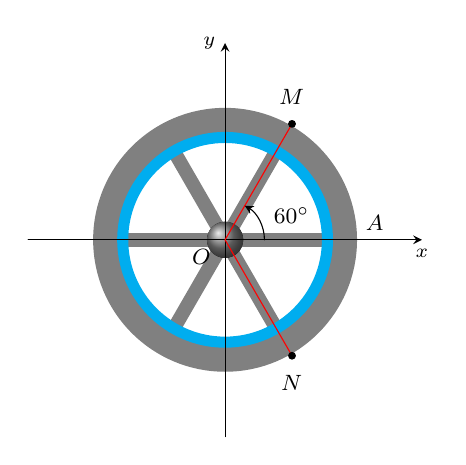
\begin{tikzpicture}[scale=1.0,font=\footnotesize,line join=round,line cap=round,>=stealth];
		\draw[line width=5,color=gray]  (0:0)--(60:1.3);
		 \draw[line width=5,color=gray] (0:0)--(120:1.3);
		\draw[line  width=5,color=gray] (0:0)--(180:1.3);
		\draw[line  width=5,color=gray] (0:0)--(240:1.3);
		\draw[line width=5,color=gray]  (0:0)--(300:1.3);
		 \draw[line width=5,color=gray] (0:0)--(360:1.3);
		\draw[line width=10,gray] (0:1.5)  arc (0:360:1.5);
		\draw[line width=4,color=cyan]  (0:1.3) arc (0:360:1.3);
		\fill[ball color=gray] (0:0)  circle (.23);
		\draw[->]  (-2.5,0) -- (2.5,0) node[below] {\scriptsize $x$};
		\draw[->] (0,-2.5) -- (0,2.5) node[left]  {\scriptsize $y$};
		\draw (1.9,0) node[above]  {$A$};
		\draw  (-0.3,0) node[below] {$O$};
		\draw (65:2)  node {$M$};
		 \draw (-65:2) node {$N$};
		 \draw[color=red] (0:0)--(60:1.7)
			 (0:0)--(-60:1.7);
		\draw  (20:0.9) node{$60^\circ$};
		\draw[-stealth] (0:.5) arc (0:60:.5); 
		\draw[fill=black]  (-60:1.7) circle (1.2pt)
			 (60:1.7) circle (1.2pt);
	\end{tikzpicture}
		} 
	\loigiai{ 
		Dựa vào hình vẽ, số đo tổng quát của góc lượng giác  $(Ox, ON)=-60+k\cdot 360^\circ$, $k\in\mathbb{Z}$.
	} 
\end{ex}

% nguồn: Ok_Toan11_TracNghiem_Lan2
\begin{ex}%[1D1H1-6]%[ma:83f70afa]
	\immini[thm]{Trong hình vẽ dưới đây, chiếc quạt có ba cánh được  phân bố đều nhau. Số đo của góc lượng giác $(Ox, ON)$ bằng
	\choice 
		{$50^{\circ}+k  360^{\circ}$ $(k \in \mathbb{Z})$}
		{$120^{\circ}+k  360^{\circ}$ $(k \in \mathbb{Z})$}
		{\True $70^{\circ}+k  360^{\circ}$ $(k \in \mathbb{Z})$}
		{$-70^{\circ}+k 360^{\circ}$ $(k \in \mathbb{Z})$}} 
		{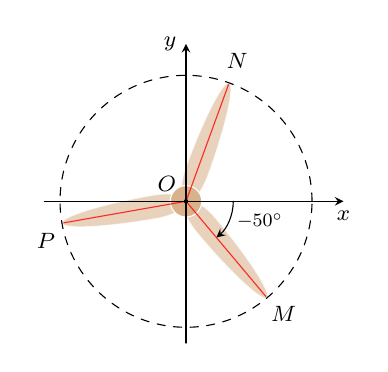
\begin{tikzpicture}[>=stealth,line join=round,line cap=round,font=\footnotesize,scale=0.8]
		\def\star t{-20} 
		\foreach \i/\p  in {\star t + 90/N,\star t + 210/P,\star t + 330/M}{
			\path [fill=brown!50,opacity=0.7,draw=white,rotate=\i] 
			 (.5,-.1875)
			 arc (270:90:.5 and 0.1875)
			arc (90:-90:1.5  and 0.1875);
			\path (\i:1.97)  coordinate (\p);
		} 
		\path  (0,0) coordinate (O);
		 \path[fill=brown!60,opacity=1,draw=white] (0,0) circle [radius=.25];
		\draw[dashed] (0,0) circle  (2cm);
		\draw[red,opacity=0.8]  (O)--(N)
			 (O)--(M)
			(O)--(P); 
		\draw[->] (-2.25,0)--(2.5,0)  node[below]{$x$};
		\draw[->] (0,-2.25)--(0,2.5)  node[left]{$y$};
		\fill (0,0) circle  (1pt) node[above left] {$O$};
		\foreach \l/\g in {N/70,M/-45,P/-135} 
		\draw[fill=black] (\l)  +(\g:.4) node{$\l$};
		 \draw[->] (0:0.75) arc (0:-50:0.75) node[pos=0.5,right,scale=0.85]{$-50^\circ$};
	\end{tikzpicture}
		} 
	\loigiai{ 
		 Vì ba cánh quạt phân bố đều nhau nên ta suy ra $\widehat{MON}=\widehat{NOP}=\widehat{POM}=120^{\circ}$.\\
		 Suy ra một góc lượng giác $(OM, ON)$ có số đo là $120^{\circ}$.\\
		Theo hình vẽ, ta có một góc lượng giác $(Ox, OM)$ có số đo  là $-50^{\circ}$.\\
		 Theo hệ thức Chasles, ta suy ra
		\[\text{sđ}(Ox, ON)=\text{sđ}(Ox, OM)+\text{sđ}(OM, ON)+k 360^{\circ}=-50^{\circ}+120^{\circ}+k 360^{\circ}=70^{\circ}+k 360^{\circ}(k  \in \mathbb{Z}).\]
	} 
\end{ex}

% nguồn: Ok_TracNghiemLop11_Lan1
\begin{ex}%[1D1V1-6]%[ma:a89a477d]
	Một bánh xe quay theo chiều  dương được $5$ vòng trong $8$ giây. Trong $3$ giây bánh xe quay được một góc lượng giác có số đo là bao nhiêu
	\choice 
		{$\dfrac{3}{4} \pi$} 
		{$\dfrac{48}{5}  \pi$}
		 {\True $\dfrac{15}{4} \pi$}
		{$\dfrac{5}{6}  \pi$}
	\loigiai{ 
		Trong $3$ giây bánh xe quay được  $\dfrac{5\cdot 3}{8}=\dfrac{15}{8}$ vòng.\\
		Bánh xe quay  $1$ vòng được một góc là $2\pi$.\\
		Vậy bánh xe quay $\dfrac{15}{8}$ vòng được $1$ góc là $2\pi \cdot \dfrac{15}{8}=\dfrac{15}{4}  \pi$.
	} 
\end{ex}

% nguồn: Ok_TracNghiemLop11_Lan1
\begin{ex}%[1D1V1-6]%[ma:a7491148]
	Một đồng hồ treo  tường có kim giờ dài $10{,}57$ cm. Trong $30$ phút mũi kim giờ vạch lên cung tròn có độ dài bằng bao nhiêu?
	\choice 
		{\True $\dfrac{1057}{1200}  \pi$ (cm)}
		{$\dfrac{1057}{2400} \pi$  (cm)}
		{$\dfrac{1057}{600}  \pi$ (cm)}
		 {$\dfrac{1057}{4800} \pi$ (cm)}
	\loigiai{ 
		Trong $1$ giờ mũi kim giờ vạch lên $1$ cung có số  đo là $\dfrac{2\pi}{12}=\dfrac{\pi}{6}$ nên trong $30$ phút kim giờ vạch lên $1$ cung có số đo là $\dfrac{1}{12} \pi$.
		Vậy độ dài cung tròn mà mũi kim giờ vạch là  $l=R\alpha=10{,}57\times \dfrac{\pi}{12}=\dfrac{1057}{1200} \pi$
	} 
\end{ex}

% nguồn: Ok_TracNghiemLop11_Lan1
\begin{ex}%[1D1C1-6]%[ma:b9d4e761]
	Bánh xe đạp có đường kính $55$ cm (kể cả lốp). Nếu chạy với vận tốc $40$ km/h thì trong $25$ s bánh xe quay được số vòng gần bằng với  kết quả nào dưới đây?
	\choice 
		 {$52$}
		{\True  $161$}
		 {$322$}
		 {$200$}
	 \loigiai{
		 Ta có $\heva{&r=\dfrac{55}{2} \text{ cm} = \dfrac{0,55}{2} \text{ m}\\ & v = 40 \text{ km/h} = \dfrac{40000}{3600} \text{ m/s}}$ \\
		Gọi $l$ là quãng đường đi được trong  $25$ giây.\\
		Gọi $x$ là số vòng bánh xe  quay được trong $25$ giây.\\
		Khi đó $l=2\pi\cdot r  \cdot x$\\
		Mà $l=\dfrac{25\cdot40000}{3600}=\dfrac{2500}{9}$  suy ra $x=\dfrac{l}{2\pi \cdot r}=160{,}7\approx 161$ (vòng).
	 }
\end{ex}


%%%%%%%%%%%%%%%% ĐÚNG/SAI %%%%%%%%%%%%%%%%

% nguồn: Ok_dungsai_lop11_Lan1
\begin{ex}%[1D1H1-6]%[ma:f334a70a]
 \immini{Trong hình vẽ bên, ta xem hình ảnh đường tròn trên một bánh lái tàu thuỷ tương ứng với một đường tròn lượng giác. Các mệnh đề  sau \textbf{ĐÚNG} hay \textbf{SAI} ?
 \choiceTF 
  {\True Công thức tổng quát biểu diễn góc lượng giác $(OA,OB)$ theo đơn vị radian: $(OA,OB)=\dfrac{\pi}{4}+k2\pi \,  (k\in \mathbb{Z})$}
  {Công thức tổng quát chỉ ra góc lượng giác  tương ứng với bốn điểm biểu diễn là $A$, $C$, $E$, $G$ theo đơn vị radian là $k\dfrac{\pi}{3} (k\in \mathbb{Z})$}
  {\True Công thức tổng quát chỉ ra góc lượng giác tương ứng  với hai điểm biểu diễn là $A$, $E$ theo đơn vị độ là $k180 ^{\circ} (k\in \mathbb{Z})$}
  {Công thức tổng quát biểu diễn góc lượng giác $(OA,OC)+(OC,OH)$ theo đơn vị radian là $\dfrac{\pi}{4}+k2\pi (k\in  \mathbb{Z})$}
  } 
   {
  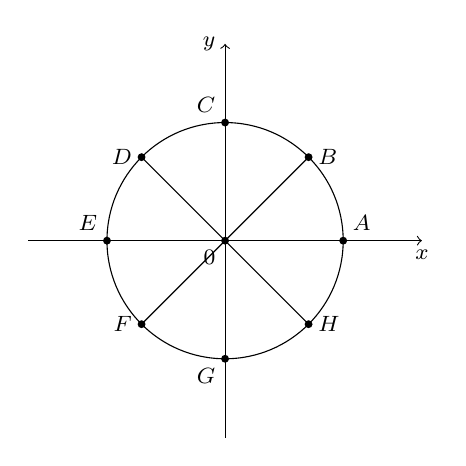
\begin{tikzpicture}[font=\footnotesize]
    \draw[->] (180:2.5)--(0:2.5) node[below]  {$x$};
    \draw[->] (-90:2.5)--(90:2.5) node[left] {$y$}; 
    \draw  (0:0) circle (1.5);
    \fill (0:0) circle (0.05)  node[below left] {$0$};
    \fill (45:1.5) circle (0.05)  node[right] {$B$};
    \fill (-45:1.5) circle (0.05) node[right] {$H$}; 
     \fill (135:1.5) circle (0.05) node[left] {$D$};
    \fill (225:1.5) circle (0.05)  node[left] {$F$};
     \fill (0:1.5) circle (0.05) node[above right] {$A$};
    \fill  (180:1.5) circle (0.05) node[above left] {$E$};
    \fill (90:1.5) circle (0.05)  node[above left] {$C$};
    \fill (-90:1.5) circle (0.05) node[below left] {$G$}; 
     \draw (0:0)--(45:1.5);
    \draw (0:0)--(135:1.5); 
    \draw  (0:0)--(225:1.5);
    \draw (0:0)--(-45:1.5); 
   \end{tikzpicture}
  } 
  \loigiai{
  \begin{itemchoice}
    \itemch Ta có $(OA,OB)=\dfrac{\pi}{4}+k2\pi \, (k\in \mathbb{Z})$.
   \itemch Ta thấy $A$, $C $, $E$, $G$ lần lượt biểu diễn cho các góc lượng giác $0$ rad, $\dfrac{\pi}{2}$ rad, $\pi$ rad, $\dfrac{3\pi}{2}$ rad, $2\pi$ rad, $\dfrac{5\pi}{2}$ rad, $\ldots$ Tất cả các góc này theo thứ tự chênh lệch nhau $\dfrac{\pi}{2}$ rad. Vì vậy công thức duy nhất biểu  diễn cho các góc lượng giác ấy là $k\dfrac{\pi}{2}\, (k\in \mathbb{Z})$.
   \itemch Ta thấy hai điểm $A,E$ lần lượt biểu diễn cho các góc lượng giác $0 ^{\circ}$, $180 ^{\circ}$, $360 ^{\circ}$, $540 ^{\circ}, \ldots$ Tất cả các góc này theo thứ tự chênh lệch  nhau $180 ^{\circ}$. Vì vậy công thức duy nhất biểu diễn cho các góc lượng giác ấy là $k180 ^{\circ}\, (k\in \mathbb{Z})$.
   \itemch  Theo hệ thức Sa-lơ, ta có
   \[\begin{array}{l}{(OA,OB)+(OB,OC)=(OA,OC)=\dfrac{\pi}{2}+k2\pi \, (k\in \mathbb{Z}).} \\ {(OA,OC)+(OC,OH)=(OA,OH)=-\dfrac{\pi}{4}+k2\pi \, (k\in \mathbb{Z}).}
  \end{array}
  \] 
 \end{itemchoice}
} 
\end{ex}

% nguồn: Ok_dungsai_lop11_Lan2
\begin{ex}%[1D1H1-6]%[ma:21efe57e]
	Trong hình vẽ dưới đây, ta xem hình ảnh đường tròn trên một  bánh lái tàu thuỷ tương ứng với một đường tròn lượng giác.
	\begin{center}
	 \definecolor{cadmiumgreen}{rgb}{0.0, 0.42, 0.24}
		\newcommand{\vekimtonua}[3]{ 
		 \draw[fill=cadmiumgreen,draw=none] ($(0,0)+(#3:#1)$)--($(0,0)+(#3-90:#2)$)--(0,0)--cycle;
		\draw[fill=cadmiumgreen,draw=none,rotate=180]  ($(0,0)+(#3:#1)$)--($(0,0)+(#3-90:#2)$)--(0,0)--cycle;
		\draw[fill=yellow,draw=white]  ($(0,0)+(#3:#1)$)--($(0,0)+(#3+90:#2)$)--(0,0)--cycle;
		\draw[fill=yellow,draw=white,rotate=180]  ($(0,0)+(#3:#1)$)--($(0,0)+(#3+90:#2)$)--(0,0)--cycle;
		} 
		\begin{tikzpicture}[line cap=round,declare function={r1=0.18; r2=1.65;}]
				\path[fill=brown!65!black,even  odd rule] (0,0) circle ({r2-r1}) circle (r2);
				\foreach \i in {0,45,...,315}{ 
					\path[fill=brown!85!black,draw,rotate=\i]  (70:{3*r1})--++(0,r1) arc (0:90:0.1)
					--+(0,0.6)  arc (-90:0:0.1)
					 --+(0,0.45) arc (0:90:0.1)
					--+(0,0.4) arc  (0:180:0.1)
					--+(0,-0.4)  arc (90:180:0.08)
					--+(0,-0.45)  arc (180:270:0.1)
					--++(0,-0.62) to[out=180,in=90]+(-0.1,-0.1) 
					--(111:{3*r1})--cycle; 
				} 
				\path[fill=orange!35!white,even  odd rule] (0,0) circle ({2*r1}) circle (3*r1);
				\path[fill=orange!45!white,even odd  rule] (0,0) circle (r1) circle (2*r1);
				\path[fill=brown,even odd rule] (0,0) circle  (r2) circle ({1.5*r1+r2});
				\draw (0,0)  circle ({2*r1}) circle (3*r1)
					circle (r2) circle  ({1.5*r1+r2});
				 \foreach \i/\d in {0/A,1/B,2/C,3/D,4/E,5/F,6/G,7/H}
					{\path ({45*\i}:{1.5*r1+r2}) coordinate (\d);} 
				 \path (0,0)
					(0:r2) coordinate  (0);
				\foreach  \t/\g in {A/45,B/0,C/45,D/90,E/150,F/-150,G/-150,H/45}{
					\fill (\t) circle (1pt) node[shift={(\g:11pt)}]{$\t$}; 
				 }
				 \newcommand\bigangle[2][]{
				 \draw[->,domain=0:#2,variable=\t,samples=200,>=latex,#1]
					plot ({0.25*(\t+6*#2)*cos (\t)/(2*#2)}, 
					{0.25*(\t+  6*#2)*sin (\t)/(2*#2)});
				 }
			\end{tikzpicture}
	\end{center}
	 \choiceTF
		{\True Công thức tổng quát biểu diễn góc lượng giác $(OA,OB)$ theo đơn vị radian là  $(OA,OB)=\dfrac{\pi}{4}+k2\pi$ $(k\in \mathbb{Z})$}
		{Công thức tổng quát chỉ ra  góc lượng giác tương ứng với bốn điểm biểu diễn là $A, C, E, G$ theo đơn vị radian là $k\dfrac{\pi}{3}$ ($k\in \mathbb{Z}$)}
		{\True Công thức tổng quát chỉ ra góc lượng giác tương ứng với hai điểm biểu diễn là $A, E$ theo đơn vị độ là $k 180^\circ$  ($k \in \mathbb{Z}$)}
		{Công thức tổng quát biểu diễn góc lượng giác $(OA,OC)+(OC,OH)$ theo đơn vị radian  là $\dfrac{\pi}{4}+k2\pi$ $(k\in \mathbb{Z})$}
	 \loigiai{
		\begin{itemchoice}
			 \itemch \textbf{Đúng.}\\
			 Ta có $(OA,OB)=\dfrac{\pi}{4}+k2\pi$ $(k\in \mathbb{Z})$.
			 \itemch \textbf{Sai.}\\
			Ta thấy $A$, $C$, $E$, $G$ lần lượt biểu diễn cho các góc  lượng giác $0$ rad, $\dfrac{\pi}{2}$ rad, $\pi$ rad, $\dfrac{3 \pi}{2}$ rad, $2\pi$ rad, $\dfrac{5 \pi}{2}$ rad, \dots. Tất cả các góc này theo thứ tự chênh lệch nhau $\dfrac{\pi}{2}$ rad. Vì vậy công thức duy nhất biểu diễn cho các góc lượng giác ấy là $k\dfrac{\pi}{2}$ $(k \in \mathbb{Z})$.
			\itemch  \textbf{Đúng.}\\
			Ta thấy hai điểm $A$, $E$ lần lượt biểu diễn cho các góc lượng giác $0^\circ$, $180^\circ$, $360^\circ$, $540^\circ$, \ldots. Tất cả các góc này theo thứ tự chênh lệch  nhau $180^\circ$. Vì vậy công thức duy nhất biểu diễn cho các góc lượng giác ấy là $k 180^\circ$ $(k \in \mathbb{Z})$.
			\itemch \textbf{Sai.}\\ 
			Theo hệ thức  Sa-lơ, ta có
			$$\begin{aligned}
			& (O A, O B)+(O B,  O C)=(O A, O C)=\dfrac{\pi}{2}+k 2 \pi(k \in \mathbb{Z}) \\
			& (O A, O C)+(O C, O H)=(O A,  O H)=-\dfrac{\pi}{4}+k 2 \pi(k \in \mathbb{Z})
		\end{aligned}$$
	\end{itemchoice}
} 
\end{ex}

% nguồn: Ok_dungsai_lop11_Lan2
\begin{ex}%[1D1H1-6]%[ma:96d08849]
	Một vận động viên đi xe đạp trên đường,  bánh xe đạp của vận động viên này quay được $11$ vòng trong $5$ giây. Biết rằng đường kính của bánh xe đạp là $680$ mm.
	\begin{center}
		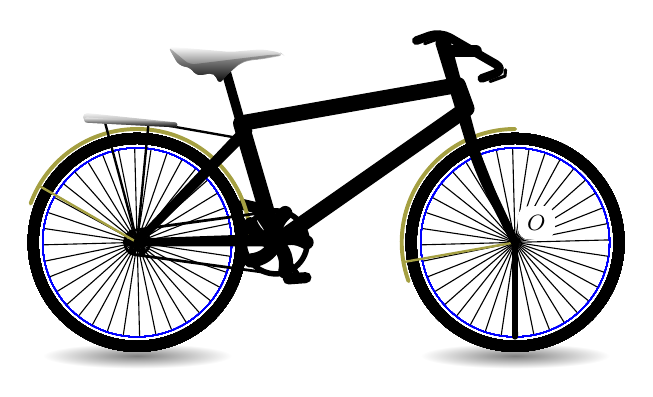
\begin{tikzpicture}[scale=0.8,font=\footnotesize,line join=round,line cap=round,>=stealth]
				 \shade[shading=radial] (-1.5,-2) rectangle (1.5,-1.6);
				 \shade[shading=radial] (4.5,-2) rectangle (7.5,-1.6);
				\def\Radius{1.5cm} 
				 \foreach \a in {0,10,...,350}{
					\draw[black] (0,0)  -- (\a+1.5:\Radius);
					\draw[blue]  (0,0) circle[radius=\Radius];
					\draw[line width=4pt] (0,0) circle[radius=\Radius+0.15cm]; 
				} 
				\foreach \h in  {0,60,...,300}{
					\draw[color=black,line width=0.5mm,rotate around={\h:(0,0)}] (0,0) edge[-,bend left=40] (0.2cm,0) edge[-,bend right=40] (0.2cm,0);
				 }
				\draw[line width=1pt] (0,0)  circle[radius=0.2cm];
				\draw[line width=4pt,rounded corners=1pt,rotate=0]  (1.68,0.6)--(1.94,0.54);
				\draw[line width=0.3mm,yellow!60!black]  (1.8,0) arc (0:150:1.8cm)--(0,0);
				\draw[line width=0.5mm,yellow!60!black] (1.8,0) arc (0:160:1.8cm); 
				\foreach \b in  {0,10,...,350}{
					\draw[black,rotate around={\b+1.5:(6,0)}] (6,0) -- (7.5,0); 
					\draw[blue] (6,0) circle[radius=\Radius]; 
					\draw[line width=4pt] (6,0)  circle[radius=\Radius+0.15cm];
				} 
				\draw[black,line width=2pt] (6,0)  node[above right,fill=white,rounded corners]{$O$}--++ (-90:1.5);
				\draw[line width=0.3mm,yellow!60!black]  (6,1.8) arc (90:190:1.8cm)--(6,0);
				\draw[line width=0.5mm,yellow!60!black]  (6,1.8) arc (90:200:1.8cm);
				 \draw[line width=1pt] (0,0.2cm)--(2.2,0.5cm)
					(0,-0.2cm)--(2.2,-0.5cm); 
				\draw[line width=2pt] (2.2,0)--(2.6,-0.6) 
					(2.2,0)--(1.8,0.6); 
				\draw[line width=1mm,rounded  corners=8pt,rotate around={25:(6,0)}] (6,0)--(6,1.3cm)--++(80:2.1cm);
				\draw[line width=1mm,rounded corners=8pt,rotate around={27:(6,0)}] (6,0)--(6,1.3cm)--++(80:2.1cm); 
				\draw[line width=1mm,rounded corners=8pt,rotate around={26:(6,0)}] (6,0)--(6,1.3cm)--++(80:2.1cm) coordinate (a); 
				\draw[line width=1.5mm]  (a)--++(-80:0.15cm)--++(0:0.5cm)--++(180:0.05cm) coordinate (b);
				\draw[line width=1.1mm,rounded corners=4pt] (b)--++(-30:0.6cm) coordinate  (c)--++(-160:0.4cm)
					(b)--++(150:0.6cm) coordinate (d)--++(200:0.4cm); 
				\draw[line width=0.4mm,rounded  corners=0pt] (c)--++(-95:0.1cm)--++(-160:0.25cm)
					 (d)--++(-95:0.1cm)--++(200:0.25cm);
				\draw[line width=2mm,rotate around={35:(2.2,0)}] (2.2,0)--++(3.7,0)--++(75:0.4cm)--++(155:3.5) coordinate (e)--(2.2,0); 
				\draw[line  width=1mm] (0,0)--(2.2,0)
					(0,0)--(45:2.5cm) 
					(0,0)--(46.5:2.5) 
					 (0,0)--(2:2.2);
				\draw[line width=1.2mm] (e)--++(106:0.9cm)--++(-74:0.1cm)  coordinate (d);
			\foreach \c in {0,72,...,288}{\draw[line width=1.8mm,rotate around={\c:(2.2,0)}] (2.2,0) edge[-,bend left=30] (2.69,0);}
			\draw[line  width=2pt] (2.2,0) circle[radius=0.5cm];
			\fill (2.2,0)  circle[radius=0.1cm];
			\draw[line width=4pt,rounded corners=1pt,rotate=0]  (2.4,-0.58)--(2.68,-0.56);
			 \draw[line width=2pt] (2.2,0)--(2.6,-0.6);
			\shade[top color=white,bottom color=black,rounded corners=2pt,rotate around={10:(d)}]  (d)--++(220:2mm)--++(100:2mm)--++(180:3mm)--++(110:1.5mm)--++(160:2mm)--++(110:3.5mm) coordinate (i)--++(-15:10mm)--++(-5:5mm)--++(-20:3mm) coordinate (j)--++(-50:0.7mm)--++(180:4mm)--++(170:1mm)--++(-175:2mm)--(d);
			\shade[top color=gray!50,bottom  color=black,rounded corners=2pt,rotate around={10:(d)}] (d)--++(220:2mm)--++(100:2mm)--++(180:3mm)--++(110:1.5mm)--++(160:2mm)--++(110:3.5mm)--++(-50:4.5mm)--++(-3:13mm)--++(-10:2mm)--++(180:4mm)--++(170:1mm)--++(-175:2mm)--(d);
			\filldraw[black]  (0,0) circle (1pt)
				(6,0) circle  (1pt);
			\draw[line width=0.3mm] (0,0)--++(105:2cm)--++(-2:0.7cm) coordinate (g)--+(-10:1.5cm) 
				(g)--(0,0); 
			\shade[top color=gray!10!white,bottom color=gray] (-0.8cm,1.9cm)--++(-3:1.4cm) arc (-90:90: 0.4mm)--++(174:1.4cm)  arc (90:270: 0.65mm);
			\shade[top color=gray!20,bottom color=black] (-0.8cm,1.9cm)--++(-3:1.4cm) arc (-90:90: 0.4mm)--++(177:1.4cm)  arc (90:270: 0.4mm);
		\end{tikzpicture}
	\end{center}
	 \choiceTF
		{\True Góc (theo độ rađian) mà bánh xe quay được trong $1$ giây  là $792^{\circ}$}
		{Góc (theo rađian) mà bánh xe quay được trong $1$ giây  là $\dfrac{2\pi}{5}(\mathrm{rad})$}
		{Trong một  phút bánh xe quay được $130$ vòng}
		{\True Quãng đường mà người đi xe đã đi được trong $1$ phút khoảng  $282$ m}
	 \loigiai{
		\begin{itemchoice}
			\itemch Trong $1$  giây, bánh xe đạp quay được $\dfrac{11}{5}$ vòng.\\
			Vì một vòng ứng với góc bằng $360^{\circ}$ nên  góc mà bánh quay xe quay được trong $1$ giây là
			 $\dfrac{11}{5} \cdot 360=792^{\circ}$.
			\itemch Vì một vòng ứng với góc bằng $2\pi$ nên góc mà bánh quay xe  quay được trong $1$ giây là
			$\dfrac{11}{5} \cdot 2\pi=\dfrac{22\pi}{5}$ rad. 
			\itemch Ta có $1$ phút $=60$  giây.\\
			Trong $1$ phút bánh xe quay được $60\cdot \dfrac{11}{5}=132$  vòng.
			\itemch Chu vi  của bánh xe đạp là $C=680\pi$ mm.\\
			Quãng đường mà người đi xe đạp  đã đi được trong một phút là $S=132\cdot 680\pi \approx 282$ m.
		\end{itemchoice}
	} 
\end{ex}

% nguồn: Ok_dungsai_lop11_Lan2
\begin{ex}%[1D1H1-6]%[ma:0c219cdb]
	Từ một vị trí ban đầu trong không gian, vệ tinh $X$ chuyển động theo  quỹ đạo là một đường tròn quanh Trái Đất và luôn cách tâm Trái Đất một khoảng bằng $9\,200$ km. Sau $2$ giờ thì vệ tinh $X$ hoàn thành hết một vòng di chuyển.
	\choiceTF 
		{\True Quãng đường vệ  tinh $X$ chuyển động được sau $1$ giờ là $\approx 28902{,}65\mathrm{~km}$}
		{\True Quãng đường vệ tinh $X$ chuyển động  được sau $1{,}5$ giờ là $\approx 43353{,}98\mathrm{~km}$}
		{Sau khoảng $5{,}3$ giờ thì $X$ di chuyển được quãng đường  $240\,000$ km}
		{\True Giả sử vệ tinh di chuyển theo chiều dương của đường  tròn, sau $4{,}5$ giờ thì vệ tinh vẽ nên một góc $\dfrac{9\pi}{2} \mathrm{rad}$}
	 \loigiai{
		\begin{itemchoice}
			\itemch  Một vòng di chuyển của $X$ chính là chu vi đường tròn
			 $$
			C=2\pi R=2\pi\cdot 9\,200=18\,400 \pi\,\mathrm{km}. 
			$$ 
			Sau  1 giờ, vệ tinh di chuyển nửa đường tròn với quãng đường là
			$$ 
			\dfrac{1}{2} C=9\,200 \pi  \approx 28\,902{,}65\,\mathrm{km}.
			 $$
			\itemch Sau 1,5 giờ, vệ tinh  di chuyển được $\dfrac{1,5.1}{2}$ đường tròn (hay $\dfrac{3}{4}$ đường tròn), quãng đường là $\dfrac{3}{4} C=\dfrac{3}{4} \cdot 18400\pi=13800\pi \approx 43353,98(\mathrm{~km})$.
			\itemch Số giờ để vệ tinh $X$ thực hiện quãng đường 240000 km là  $\dfrac{240\,000}{9\,200\pi} \approx 8{,}3$ (giờ).
			\itemch Sau 4,5 giờ thì số vòng tròn mà vệ tinh $X$ di chuyển được là $\dfrac{4,5}{2}=\dfrac{9}{4}$  (vòng).\\
			Số  đo góc lượng giác thu được là $\dfrac{9}{4}.2\pi=\dfrac{9\pi}{2} \,\mathrm{rad}$.
		\end{itemchoice}
	} 
\end{ex}


%%%%%%%%%%%%%%%% TRẢ LỜI NGẮN %%%%%%%%%%%%%%%%

% nguồn: Ok_TraLoiNgan_Lop11_Lan2
\begin{ex}%[1D1H1-6]%[ma:c2ca0962]
	Một đồng hồ treo tường, kim giờ dài $10{,}57$ cm và kim phút dài $13{,}34$ cm. Trong $30$ phút mũi kim giờ vạch lên cung tròn có độ dài bằng bao nhiêu? (Kết quả làm tròn đến hàng phần  trăm).
	 \shortans{2,77}
	\loigiai{ 
		Ta có giờ thì kim giờ vạch lên 1 cung có số đo $\pi$ nên 30 phút kim giờ vạch lên 1 cung có số đo là $\dfrac{1}{12} \pi$, suy ra độ dài cung tròn mà nó vạch lên  là $l=R\alpha=10{,}57\cdot \dfrac{3{,}14}{12} \approx 2{,}77$ cm.
	 }
\end{ex}

% nguồn: Ok_TraLoiNgan_Lop11_Lan2
\begin{ex}%[1D1H1-6]%[ma:5584938c]
	Trong chặng đua nước rút, bánh xe của một vận động viên đua  xe đạp quay được $30$ vòng trong $8$ giây. Chọn chiều quay của bánh xe là chiều dương. Xét van $V$ của bánh xe.
	Sau $1$ phút, van $V$ đó quay được  một góc có số đo bao nhiêu radian (làm tròn đến hàng đơn vị)?
	\shortans{1414} 
	 \loigiai{
		Sau $1$ giây, van  $V$ của bánh xe quay được $\dfrac{30}{8}=3{,}75$ (vòng).\\
		Sau $1$ phút, van  $V$ của bánh xe quay được $3{,}75\cdot 60=225$ (vòng).\\
		Suy ra sau $1$ phút, van $V$ của bánh xe quay được một góc có số  đo là $225\cdot 2\pi=450\pi\approx 1414$.
	} 
\end{ex}

% nguồn: Ok_TraLoiNgan_Lop11_Lan2
\begin{ex}%[1D1H1-6]%[ma:5b5954fd]
	Một chiếc quạt trần năm cánh quay với tốc độ $175$ vòng trong một phút. Chọn chiều quay của quạt là chiều dương. Sau thời gian bao lâu cánh quạt quay được một góc có số đo $42\pi$? 
	\shortans{7,2} 
	\loigiai{ 
		Sau $1$  giây, cánh quat quay được $\dfrac{175}{60}=\dfrac{35}{12}$ (vòng) theo chiều dương.\\
		Suy ra sau $1$ giây, cánh quạt quay được một góc có số đo là $\dfrac{35}{12}  \cdot 2\pi=\dfrac{35\pi}{6}$.\\
		Thời gian để cánh quạt quay được một góc có số đo  $42\pi$ là $42\pi: \dfrac{35\pi}{6}=7{,}2$ giây.
	 }
\end{ex}

% nguồn: Ok_TraLoiNgan_Lop11_Lan2
\begin{ex}%[1D1H1-6]%[ma:c4c9881f]
	Một chiếc quạt trần năm cánh quay với tốc độ $45$ vòng trong một phút. Chọn chiều quay của quạt là chiều thuận. Sau $3$ giây, quạt quay được một góc có  số đo bao nhiêu radian? (Kết quả làm tròn đến hàng phần mười).
	 \loigiai{
	 \shortans{11,1}
		Trong 3 giây, quạt quay được $3\cdot  \dfrac{45}{60}=\dfrac{9}{4}$ (vòng).\\
		Vậy quạt quay dược một góc $2\pi \cdot \dfrac{9}{4}=\dfrac{9\pi}{2} \approx 11{,}1$ rad. 
	 }
\end{ex}

% nguồn: Ok_TraLoiNgan_Lop11_Lan2
\begin{ex}%[1D1H1-6]%[ma:9f6a68d5]
	Trong chặng đua nước rút, bánh xe của một vận động viên đua xe đạp quay được $30$ vòng trong $8$ giây. Chọn chiều quay của bánh xe là chiều dương. Xét van $V$ của bánh xe. Biết rằng bán kính của bánh xe là $35$ cm. Độ  dài quãng đường mà vận động viên đua xe đạp đã đi được trong $1$ phút là bao nhiêu mét (làm tròn đến hàng đơn vị)?
	\shortans{495} 
	\loigiai{ 
		Sau $1$ giây,  van $V$ của bánh xe quay được $\dfrac{30}{8}=3,75$ (vòng).\\
		Sau $1$ phút, van $V$ của bánh xe quay được $3{,}75\cdot 60=225$ (vòng).\\ 
		Suy ra sau $1$ phút, van $V$ của bánh xe quay được một góc có số đo  là $225\cdot 2\pi=450\pi$.\\
		Mỗi góc ở  tâm với số đo $1$ rad chắn một cung có độ dài bằng bán kính bánh xe $r=0{,}35$ m.\\
		Do đó độ dài  quãng đường mà vận động viên đua xe đạp đã đi được trong $1$ phút là $$
		450 \pi\cdot  0{,}35 \approx 495\, \mathrm{m}.
		$$ 
	 }
\end{ex}

% nguồn: Ok_TraLoiNgan_Lop11_Lan2
\begin{ex}%[1D1H1-6]%[ma:e56e8f56]
	Một chiếc quạt trần năm cánh  quay với tốc độ $175$ vòng trong một phút. Chọn chiều quay của quạt là chiều dương. Sau $5$ giây, cánh quạt quay được một góc có số đo bao nhiêu radian (làm tròn đến hàng phần mười)?
	\shortans{91,6} 
	 \loigiai{
		Sau $1$ giây, cánh quat  quay được $\dfrac{175}{60}=\dfrac{35}{12}$ (vòng) theo chiều dương.\\
		Suy ra sau $1$ giây, cánh  quạt quay được một góc có số đo là $\dfrac{35}{12} \cdot 2\pi=\dfrac{35\pi}{6}$.\\
		Vậy sau $5$ giây, cánh quạt quay được một góc có số đo là $\dfrac{35\pi}{6}  \cdot 5=\dfrac{175\pi}{6}=91{,}6$.
	} 
\end{ex}

% nguồn: Ok_TraLoiNgan_Lop11_Lan2
\begin{ex}%[1D1H1-6]%[ma:1e16d071]
	Khi xe đạp di chuyển, van $V$ của bánh xe quay quanh trục $O$ theo chiều kim đồng hồ với tốc độ góc không đổi là $11$ rad/s. Ban đầu van nằm ở vị trí $A$. Hỏi sau một phút di chuyển, khoảng cách từ van đến mặt đất là bao nhiêu, biết bán kính $OA=58$ cm? Giả sử độ  dày của lốp xe không đáng kể. (Kết quả làm tròn đến hàng phần mười).
	\begin{center}
		\begin{tikzpicture}[line join = round,line cap = round,scale = 1.3,transform shape]
				\clip (-3,-2.2) rectangle  (3.3,1.7);
				 \definecolor{beige}{rgb}{0.96,0.96,0.86}
				\definecolor{frenchblue}{rgb}{0.0,0.45,0.73} 
				 \definecolor{battleshipgrey}{rgb}{0.52,0.52,0.51}
				 \definecolor{earthyellow}{rgb}{0.88,0.66,0.37}
				\tikzset{xe_dap/.pic  = {
				 \draw[fill = battleshipgrey] (1.66,-.78) circle (31pt);
				\draw[fill = white]  (1.66,-.78) circle (26pt);
				\draw[fill = battleshipgrey] (-1.75,-.78) circle (31pt); 
				 \draw[fill = white] (-1.75,-.78) circle (26pt);
				 \draw[fill = battleshipgrey!40] (-.21,-1.02) circle (8pt);
				 \draw (-.21,-1.02) circle (6pt);
				\draw (-.21,-1.02)  circle (5pt);
				 \draw[fill = battleshipgrey] (-.21,-1.02) circle (2pt);
				\draw (-1.79,-.79)  circle (5pt);
				\draw (-1.79,-.79) circle  (4pt);
				\draw  (-1.77,-.94)--(-.3,-1.3)
					(-1.77,-.62)--(-.2,-.73); 
				\draw (-0.8,-.1)..controls +(120:1.05) and +(80:1.25)..(-2.95,-.7) 
					(0.45,-.65)..controls +(80:1.05) and  +(140:.5)..(2.2,.28)
					 (-1.2,.44)..controls +(110:.2) and +(-80:.28)..(-2.5,.65);
				\def\S{(-.91,1.07)--(-.72,.56)--(1.03,.72)--(.94,1.05)--(1.05,1.05) 
					..controls +(-75:.3)  and +(150:.2)..(1.68,-.76)--(1.6,-.82)
					..controls +(135:.3)  and +(-70:.2)..(1.05,.52)--(-.2,-1)--(-.27,-.9)--(.97,.6)--(-.7,.45)--(-.18,-1)--(-.315,-1)--(-.8,.4)--(-1.7,-.73
					 )--(-.35,-.9)--(-.31,-1)--(-1.87,-.8)--(-.85,.5)--(-1.05,1.07)--cycle}
				\draw[fill = frenchblue] \S; 
				 \fill[frenchblue] \S;
				 \def\Y{(-.5,1.2)
					..controls +(110:.08) and +(-10:.1)..(-1.2,1.32) 
					..controls +(-170:.4)  and +(-160:.4)..(-.85,1.1)
					 ..controls +(10:.1) and +(-60:.1)..(-.5,1.2)
				 }
				\draw[fill  = earthyellow] \Y;
				\fill[earthyellow]  \Y;
				\draw  (-1.7,-.79)--(-1.1,-1.44)
					(-1.8,-.86)--(-1.45,-1.65) 
					 (-1.74,-.86)--(-1.8,-1.7)
					(-1.8,-.86)--(-2.05,-1.65) 
					 (-1.74,-.86)--(-2.3,-1.5)
					 (-1.85,-.86)--(-2.5,-1.33)
					(-1.85,-.86)--(-2.65,-1) 
					(-1.85,-.75)--(-2.68,-.7) 
					 (-1.88,-.79)--(-2.55,-.35)
					 (-1.86,-.75)--(-2.2,0)
					(-1.75,-.7)--(-2.4,-0.13) 
					 (-1.8,-.7)--(-1.75,.15)
					 (-1.63,-.72)--(-1.05,-.17)
					(-1.5,-.75)--(-.9,-.44) 
					 (-1.77,-.85)--(-.93,-1.2); \draw (-1.75,-.7)--(-1.45,.5)
					 (-1.75,-.7)--(-2.2,.5);
				\draw[fill = battleshipgrey]  (-.14,-1)--(-.3,-1)--(-.25,-1.1)--(-.33,-1.5)--(-.45,-1.5)--(-.45,-1.6)..controls +(-15:.25) and +(-5:.25)..(-.25,-1.5)--(-.19,-1.1)--cycle;
				\draw[fill =  battleshipgrey] (-.23,-.72)--(-.18,-.5)--(-.3,-.5)--(-.28,-.4)--(0,-.4)..controls +(-5:.03) and +(-5:.2)..(-0.1,-.5)--(-.14,-.72)--cycle;
				\draw (1.72,-.78)--(2.52,-.5) 
					 (1.72,-.86)--(2.35,-.2)
					 (1.72,-.86)--(2.58,-.84)
					(1.72,-.8)--(2.48,-1.18) 
					 (1.6,-.86)--(2.3,-1.45)
					 (1.7,-.86)--(1.9,-1.65)
					 (1.6,-.86)--(1.6,-1.68)
					 (1.7,-.86)--(1.35,-1.63)
					 (1.6,-.76)--(1.05,-1.45)
					 (1.6,-.86)--(.9,-1.3)
					 (1.55,-.76)--(.77,-1)
					 (1.55,-.82)--(.74,-.7)
					(1.45,-.6)--(.83,-.38) 
					 (1.54,-.75)--(1,-.14)
					(1.63,-.74)--(1.55,.13) 
					 (1.63,-.74)--(2.1,0)
					(1.7,-.77)--(1.8,0.1); 
				 \draw[fill = black!70] (1.65,-.8) circle (2.3pt);
				 \draw (1.65,-.8) circle (5pt);
				\draw[fill = black!70] (-1.79,-.79) circle (2.3pt); 
				\draw[fill = earthyellow] (.92,1.06)..controls +(120:.15)  and +(-120:0)..(1.12,1.3)--(.85,1.45)--(.5,1.45)..controls +(120:.15) and +(-120:0)..(.5,1.58)--(.72,1.58)--(1.2,1.3)--(.7,1.6)--(.74,1.64)--(1,1.56)..controls +(-30:.5) and +(30:.3)..(1.05,1.06);
					 }}
				 \path
					 (0,0) pic[scale = 1]{xe_dap};
				 \def\xmin{0.5} \def\xmax{3.2}
				\def\ymin{-2.2} \def\ymax{.8} \draw[red,-  >] (\xmin,-.8)--(\xmax,-.8) node [above left]{\tiny $x$};
				\draw[red,- >] (1.65,\ymin)--(1.65,\ymax) node [left]{\tiny $y$}; 
				\draw[red](1.65,-.8)--(2.2,-1.5); 
				\node[red] at  (2.2,-1.5) [above]{\tiny $V$};
				\node[red] at (2.45,-.9) [above]{\tiny $A$}; 
				\node[red] at (1.65,-.8) [below left]{\tiny  $O$};
				\path  (2.5,-.9) coordinate (A)
					 (2.2,-1.5) coordinate (V)
					(1.65,-.8) coordinate  (O);
				\path (O) pic[draw,angle  radius = 0.4cm]{angle = V--O--A}node[shift = {(-22:19pt)}]{\footnotesize $\alpha$};
				 \draw[dashed] (1.65,-1.86)--(3,-1.86)
					 (1.65,-1.5)--(3,-1.5);
				\draw[red,< - >]  (2.8,-1.5)--(2.8,-1.86);
				 \node at (3,-1.8) [below left]{\tiny Mặt đất};
				\node at (2.8,-1.7)  [right]{\tiny?};
				 \path (current bounding box.south) node[below]{Hình 13};
			\end{tikzpicture}
	\end{center}
	\shortans{42,8} 
	 \loigiai{
		Sau một phút di chuyển, van $V$ quay được một góc là $-11\cdot 60=-660$ rad  do bánh xe quay cùng chiều kim đồng hồ nên tạo ra góc lượng giác có giá trị âm.\\
		Khi đó $l=58+58\cdot \sin  (-660) \approx 42{,}8$ cm.
	 }
\end{ex}

% nguồn: Ok_TraLoiNgan_Lop11_Lan2
\begin{ex}%[1D1H1-6]%[ma:9ea44e93]
	Một bánh xe có $72$ răng. Số đo góc  mà bánh xe đã quay được khi di chuyển $10$ răng là bao nhiêu?
	\shortans{50} 
	 \loigiai{
		Ta có $72$ răng có chiều dài là $2\pi  R$ nên $10$ răng có chiều dài $l=\dfrac{10.2\pi R}{72}=\dfrac{5\pi}{18} R$.\\
		Theo công thức $\ell=R\alpha \Leftrightarrow \alpha=\dfrac{\ell}{R}=\dfrac{\dfrac{5}{18} \pi R}{R}=\dfrac{5}{18} \pi$ mà $a=\dfrac{180\alpha}{\pi}=\dfrac{180\cdot \dfrac{5}{18} \pi}{\pi}=50^{\circ}$.\\ 
		 Cách khác: $72$ răng tương ứng với $360^{\circ}$ nên $10$ răng tương ứng với $\dfrac{10.360}{72}=50^{\circ}$.
	} 
\end{ex}

% nguồn: Ok_TraLoiNgan_Lop11_Lan2
\begin{ex}%[1D1H1-6]%[ma:d37b8fc7]
	\immini{Thanh $OM$ quay ngược chiều kim đồng hồ quanh gốc $O$ của nó trên một mặt phẳng thẳng đứng và in bóng vuông góc xuống mặt đất như hình bên. Vị trí ban đầu của thanh là $OA$. Hỏi độ dài bóng $O'M$ của $OM$ khi thanh quay được $\dfrac{60}{13} $ vòng là bao nhiêu, biết độ dài thanh $OM$ là $10$ cm? Kết quả làm tròn đến hàng phần mười.}{	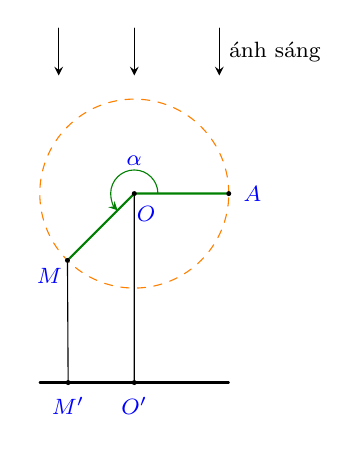
\begin{tikzpicture}[line join = round,line cap = round,>=stealth,font=\footnotesize,scale=0.6]
		\tikzset{label style/.style={font=\footnotesize}} 
		\path (0,0) coordinate  (O)
			(2,0) coordinate (A) 
			(0:0)++(225:2) coordinate  (M);
		\path (0,-4) coordinate (O') 
			(-1.4,-4) coordinate (M'); 
		\draw[orange,dashed]  (O) circle (2cm);
		\draw[rotate=0,->,green!50!black] (0.5,0) arc (0:225:0.5cm); 
		 \draw (0,0.7) node[blue] {$\alpha$};
		\draw[green!50!black,thick]  (M)--(O)--(A);
		\draw (M)--(M') 
			(O)--(O'); 
		\draw[thick] (-2,-4)--(2,-4); 
		\draw[->] (-1.6,3.5)--(-1.6,2.5); 
		\draw[->]  (0,3.5)--(0,2.5);
		\draw[->]  (1.8,3.5)--(1.8,2.5);
		\draw (1.8,3) node [right] {ánh sáng}; 
		\foreach \p/\r in  {A/0,M/220,O/-60,O'/-90,M'/-90}
		\fill  (\p) circle (1.5pt) node[shift={(\r:3mm)},blue]{$\p$};
	\end{tikzpicture}
	 }
	\shortans{7,5} 
	 \loigiai{
		Ta có $\alpha =\dfrac{60}{13} \cdot 2\pi =\dfrac{120\pi }{13}  $. Suy ra $O'M'=\left|OM\cos\alpha \right|=\left|10\cos\dfrac{120\pi }{13} \right|\approx 7{,}5$ cm.
	 }
\end{ex}

% nguồn: Ok_TraLoiNgan_Lop11_Lan2
\begin{ex}%[1D1H1-6]%[ma:8d233701]
	Trong $20$ giây bánh xe  của xe gắn máy quay được $60$ vòng. Tính độ dài quãng đường xe gắn máy đã đi được trong vòng $3$ phút với đơn vị là mét, biết rằng bán kính bánh xe gắn máy bằng $6{,}5$ cm (Kết quả làm tròn đến hàng đơn vị, lấy $\pi=3{,}14$).
	 \shortans{220}
	 \loigiai{
		Ta có $3$ phút xe đi được  $\dfrac{3\cdot 60}{20} \cdot 60=540$ vòng.\\
		Độ dài $1$ vòng bằng chu vi bánh xe là $2\pi R=2\cdot  3{,}14\cdot 6{,}5=40{,}82$ cm.\\
		Vậy quãng  đường xe đi được là $540\cdot 40{,}82=22042{,}8\,\mathrm{cm}\approx 220$ m.
	} 
\end{ex}

% nguồn: Ok_TraLoiNgan_Lop11_Lan2
\begin{ex}%[1D1H1-6]%[ma:33b9141d]
	\immini[thm]{Một cái đồng hồ treo tường có đường kính bằng $60$ cm, ta xem vành ngoài chiếc đồng hồ là một đường tròn với các điểm $A$, $B$ lần lượt tương ứng với vị trí các số $2$, $9$. Tính độ dài cung nhỏ $AB$  (Kết quả tính theo đơn vị centimét và làm tròn đến hàng phần mười).}
	{\begin{tikzpicture}[scale=0.8,font=\footnotesize,line join=round,line cap=round,>=stealth]
		\def\r{2.5} 
		 \path
			 (0,0) coordinate (O)
			(30:2.5)  coordinate (A)
			(180:2.5) coordinate (B) 
			(-30:2.5)  coordinate (C)
			(60:2) coordinate (M) 
			(-135:2) coordinate (N); 
		\draw[line width=1.5pt] (O)--(30:1) 
			 (O) circle (2pt);
		\draw[line  width=1pt] (O)--(180:2);
		\draw[line  width=2pt] (0,0) circle (3);
		\foreach \x/\g in {1/60,2/30,3/0,4/-30,5/-60,6/-90,7/-120,8/-150,9/-180,10/-210,11/-240,12/90} 
		\fill (\g:2.4) circle (1pt) 
			 ($(\g:2.7)$) node {$\x$};
		\foreach \x/\g in {A/120,B/60} 
		 \fill[black] (\x) circle (1pt)
			($(\g:3mm)+(\x)$) node  {$\x$};
	\end{tikzpicture}
	 }
	\shortans{78,5} 
	 \loigiai{
		Bán  kính đường tròn là $R=\dfrac{60}{2}=30$ cm.\\
		Ta có $\widehat{AOB}=150^{\circ}=\dfrac{150\pi}{180}\, \mathrm{rad}=\dfrac{5\pi}{6}  \,\mathrm{rad}$. \\
		Suy ra độ dài  cung nhỏ $AB$ là
		$l=R\cdot \widehat{AOB}=30\cdot \dfrac{5\pi}{6}=25\pi \approx 78{,}5$ cm. 
	} 
\end{ex}

% nguồn: Ok_TraLoiNgan_Lop11_Lan2
\begin{ex}%[1D1H1-6]%[ma:5989c328]
	Một đồng hồ treo tường, kim giờ dài $10{,}57$ cm và kim phút dài $13{,}34$ cm. Trong $30$ phút mũi kim giờ vạch lên cung tròn có độ dài là bao  nhiêu?
	\shortans{2,77} 
	\loigiai{ 
		Trong $6$ giờ thì kim giờ vạch lên $1$ cung có số đo $\pi$ nên $30$ phút kim giờ vạch lên  $1$ cung có số đo là $\dfrac{1}{12} \pi$ suy ra độ dài cung tròn mà nó vạch lên là $\ell=R\alpha=10{,}57\cdot \dfrac{3,14}{12} \approx 2{,}77$.
	} 
\end{ex}

% nguồn: Ok_TraLoiNgan_Lop11_Lan2
\begin{ex}%[1D1H1-6]%[ma:2be4e205]
	Bánh xe  đạp của người đi xe đạp quay được $2$ vòng trong $5$ giây. Hỏi trong $2$ giây, bánh xe quay được $1$ góc bao nhiêu (tính theo độ)?
	\shortans{288} 
	\loigiai{ 
		 Trong $2$ giây bánh xe đạp quay được $\dfrac{2\cdot 2}{5}=\dfrac{4}{5}$ vòng tức là quay được cung có độ dài là \[\ell=\dfrac{4}{5}\cdot 2\pi R=\dfrac{8}{5} \pi R.\]
		Ta có $\ell=R\alpha \Leftrightarrow \alpha=\dfrac{\ell}{R}=\dfrac{\dfrac{8}{5} \pi R}{R}=\dfrac{8}{5}  \pi=288^{\circ}$.
	} 
\end{ex}

% nguồn: Ok_TraLoiNgan_Lop11_Lan2
\begin{ex}%[1D1H1-6]%[ma:20b46e8f]
	Một vệ tinh được định vị tại vị trí $A$ trong không gian. Từ vị trí $A$, vệ tinh bắt đầu chuyển động quanh Trái Đất theo quỹ đạo là đường tròn với tâm là tâm $O$ của Trái Đất. Giả sử vệ tinh chuyển động hết một vòng của quỹ đạo trong $2$ h theo chiều kim  đồng hồ. Khi vệ tinh chuyển động được $3$ h, bán kính của vòng quay quét một góc lượng giác có số đo bằng bao nhiêu? (Tính theo đơn vị radian, làm tròn đến hàng phần mười).
	 \shortans{-9,4}
	 \loigiai{
		Theo giả thiết, vệ tinh chuyển động theo chiều kim đồng hồ nên sau $2$ h, bán kính của vòng quay khi vệ tinh chuyển động quét  được một góc lượng giác bằng $-2\pi$ rad.\\
		Vậy khi vệ tinh chuyển động được $3$ h thì bán kính của vòng quay quét được một góc lượng  giác bằng $-3\pi\approx -9{,}4$ rad.
	 }
\end{ex}

% nguồn: Ok_TraLoiNgan_Lop11_Lan2
\begin{ex}%[1D1H1-6]%[ma:e5f33641]
	Một bánh xe có $72$ răng. Số đo  góc mà bánh xe đã quay được khi di chuyển 10 răng là bao nhiêu?
	\shortans{50} 
	 \loigiai{
		Ta có $1$  bánh răng tương ứng với $\dfrac{360^{\circ}}{72}=5^{\circ} \Rightarrow 10$ bánh răng là $50^{\circ}$.
	 }
\end{ex}

% nguồn: Ok_TraLoiNgan_Lop11_Lan2
\begin{ex}%[1D1H1-6]%[ma:7000b280]
	Một bánh xe có đường kính kể cả lốp xe là $55$ cm. Nếu xe chạy với tốc độ $50$ km/h thì trong một giây bánh xe quay được bao nhiêu vòng? (Kết quả được làm  tròn đến hàng phần trăm).
	\shortans{8,04} 
	 \loigiai{
		Tốc độ xe là  $50\,\mathrm{km/ h} =\dfrac{50.100000}{3600}\, \mathrm{cm/s} =\dfrac{12500}{9}\, \mathrm{cm/s}$.\\
		Mỗi vòng bánh $x$ e có chiều dài $2\pi R=2\pi  \cdot \dfrac{55}{2}=55\pi(\mathrm{~cm})$.\\
		Vậy mỗi giây thì bánh  xe lăn được số vòng là $\dfrac{12500}{9}:(55\pi) \approx 8{,}04$ (vòng).
	} 
\end{ex}

% nguồn: Ok_TraLoiNgan_Lop11_Lan1
\begin{ex}%[1D1V1-6]%[ma:cc366b70]
	Một bánh xe có đường kính kể cả lốp xe là $55$ cm. Nếu xe chạy với tốc độ $50$ km$/$h thì trong một giây bánh xe quay được bao  nhiêu vòng? (Kết quả được làm tròn đến hàng phần trăm).
	\shortans{8,04} 
	 \loigiai{
		Tốc độ xe  là $50$ km$/$h $=\dfrac{50\cdot 100000}{3600}$ cm$/$s $=\dfrac{12500}{9}$ cm$/$s.\\
		Mỗi vòng bánh xe có chiều dài $2\pi R=2\pi  \cdot \dfrac{55}{2}=55\pi$ (cm).\\
		Vậy  mỗi giây thì bánh xe lăn được số vòng là $\dfrac{12500}{9}:(55\pi)\approx 8{,}04$ (vòng).
	 }
\end{ex}

% nguồn: Ok_TraLoiNgan_Lop11_Lan1
\begin{ex}%[1D1V1-6]%[ma:beec00c7]
	Trong $20$ giây bánh xe của xe gắn máy quay được $60$ vòng. Tính độ dài quãng đường xe gắn máy  đã đi được trong vòng $3$ phút, biết rằng bán kính bánh xe gắn máy bằng $0{,}65 $ dm (lấy $\pi=3{,}1416$, làm tròn đến hàng đơn vị).
	\shortans{2205} 
	\loigiai{ 
		Ta  có
		$3$ phút xe  đi được $\dfrac{3\times 60}{20} \times 60=540$ vòng.
		Độ dài $1$ vòng bằng chu vi bánh xe là $2\pi  R=2\times 3{,}1416\times 0{,}65=4{,}08408 $ (dm).
		Vậy quãng đường xe đi được là $540\times  4{,}08408=2205{,}4032$ (dm).
	 }
\end{ex}

% nguồn: Ok_TraLoiNgan_Lop11_Lan1
\begin{ex}%[1D1V1-6]%[ma:cda40c53]
	Một đồng hồ treo tường, kim giờ dài $10,57$ cm và kim phút dài $13,34$ cm. Trong $30$ phút mũi kim giờ vạch lên cung tròn có độ dài bằng  bao nhiêu? (làm tròn đến hàng phần trăm).
	\shortans{2,77} 
	 \loigiai{
		Ta có $6$ giờ thì kim giờ vạch lên $1$ cung có số đo $\pi$ nên $30$ phút kim giờ  vạch lên $1$ cung có số đo là $\dfrac{1}{12} \pi$.\\
		Suy ra độ dài cung tròn mà  nó vạch lên là $l=R\alpha=10{,}57\times \dfrac{3{,}14}{12} \approx 2{,}77$ (cm).
	} 
\end{ex}

% nguồn: Ok_TraLoiNgan_Lop11_Lan1
\begin{ex}%[1D1C1-6]%[ma:a7d4f8d8]
	Một bánh xe có đường kính kể cả lốp xe là $55$ cm. Nếu xe chạy với tốc độ $50$ km/h thì trong một giây bánh xe quay được  bao nhiêu vòng (Kết quả được làm tròn đến hàng phần trăm)?
	 \shortans{8,04}
	 \loigiai{
		Tốc độ  xe là
		$$\begin{aligned}
		 50 \text{ km/h} &= \dfrac{50\cdot100000}{3600}&& \text{ cm/s}\\
		&= \dfrac{12500}{9} &&  \text{ cm/s.}
	\end{aligned}$$
	Mỗi vòng bánh xe có chiều dài là $2\pi R=2\pi \cdot  \dfrac{55}{2}=55\pi$ (cm).\\[2pt]
	Vậy mỗi giây thì bánh xe lăn được số vòng  là $\dfrac{12500}{9}:(55\pi)\approx 8{,}04$ (vòng).
} 
\end{ex}


%%%%%%%%%%%%%%%% TỰ LUẬN %%%%%%%%%%%%%%%%

% nguồn: Ok_TuanLuan_Toan11_Lan2
\begin{ex}%[1D1H1-6]%[ma:0485f300]
	Một đồng hồ treo  tường có kim giờ dài $10{,}25$ cm, kim phút dài $13{,}25$ cm. Trong $30$ phút kim giờ vạch nên cung tròn có độ dài bao nhiêu? (làm tròn kết quả đến hàng phần trăm)
	\loigiai{ 
		Trong $6$ giờ kim giờ vạch nên một  cung có số đo là $\pi$ rad.\\
		Suy ra trong $30$ phút kim giờ vạch nên cung có số đo là $\dfrac{\pi}{12}$ rad.\\ Khi đó độ  dài cung tròn mà kim giờ vạch ra trong 30 phút là $l=R\cdot \alpha \Rightarrow l=10{,}25\cdot \dfrac{\pi}{12} \approx 2{,}68$ cm.
	} 
\end{ex}

% nguồn: Ok_TuanLuan_Toan11_Lan2
\begin{ex}%[1D1H1-6]%[ma:02bf37e2]
	Một bánh xe có đường kính bằng $60$ cm. Nếu xe chạy với vận tốc $50$ km/h thì trong $5$ giây bánh xe quay  được bao nhiêu vòng? (làm tròn kết quả đến hàng đơn vị)
	 \loigiai{
		Chu vi của bánh xe là $0{,}6\pi$  (m).\\
		Sau  $1$ giây bánh xe quay được $\left[\dfrac{50\cdot 1\,000}{3\,600}:(0{,}6\pi)\right]=\dfrac{625}{27\pi}$ (vòng).\\
		Suy ra sau $5$ giây bánh xe quay được $5\cdot \dfrac{625}{27\pi} \approx 37$  (vòng).
	} 
\end{ex}

% nguồn: Ok_TuanLuan_Toan11_Lan2
\begin{ex}%[1D1H1-6]%[ma:add23121]
	Trong $20$ giây bánh xe của xe gắn máy quay được $60$ vòng. Tính độ  dài quãng đường xe gắn máy đã đi được trong vòng $3$ phút,biết rằng bán kính bánh xe gắn máy bằng $6{,}5$ cm.
	\loigiai{ 
		 Trong $3$ phút xe đi được $\dfrac{3\cdot 60}{20}\cdot 60=540$ vòng.\\
		Độ dài $1$  vòng bằng chu vi bánh xe là $2\pi R=2\cdot 3{,}1416\cdot 6{,}5=40{,}8408$.\\
		Vậy quãng đường xe đi  được là $540\cdot 40{,}8408=22\,054{,}032$ cm.
	 }
\end{ex}
